\nsection{Turtle Graphics}

\subsection*{History}
Many attempts have been made to create programming languages
which are intuitive and easy to learn.
One of the best of these was {\it LOGO} which allowed
children as young as 3 to learn a computer language.
A subset of this language involved a ``turtle'' which
could be driven around the screen using simple instructions.

\subsection*{An Example}
At its most basic, the turtle is driven by simple instructions 
such as \verb^FORWARD^ to move the turtle and leave a trail behind it,
and \verb^RIGHT^ which rotates the turtle clockwise~:
\begin{codesnippet}
START
  FORWARD 5
  RIGHT 45
  FORWARD 5
  RIGHT 45
  FORWARD 5
  RIGHT 45
  FORWARD 5
  RIGHT 45
  FORWARD 5
  RIGHT 45
  FORWARD 5
  RIGHT 45
  FORWARD 5
  RIGHT 45
  FORWARD 5
  RIGHT 45
END
\end{codesnippet}
\begin{center}

\includegraphics[clip,trim=10cm 11cm 5cm 11cm,scale=1.25]{../Pictures/out_octagon1.pdf}
\end{center}

\noindent This may be simplified by using a loop to repeat an operation
several times.  Here our grammar allows a variable to iterate over each
item in a list~:

% octagon
\begin{codesnippet}
START
  LOOP A OVER { 1 2 3 4 5 6 7 8 }
    FORWARD 5
    RIGHT 45
  END
END
\end{codesnippet}

Here the actual values of the variable \verb^A^ weren't really important since
the variable wasn't used directly inside the loop itself.
Colours can be set by using string constants such as \verb^"RED"^ or \verb^"CYAN"^~:

% tunnel
\begin{codesnippet}
START
  LOOP D OVER { 1 2 3 4 5 6 7 8 }
    LOOP C OVER { "RED" "GREEN" "YELLOW" "BLUE" }
      COLOUR $C
      FORWARD $D
      RIGHT 90
    END
  END
END
\end{codesnippet}
\begin{center}
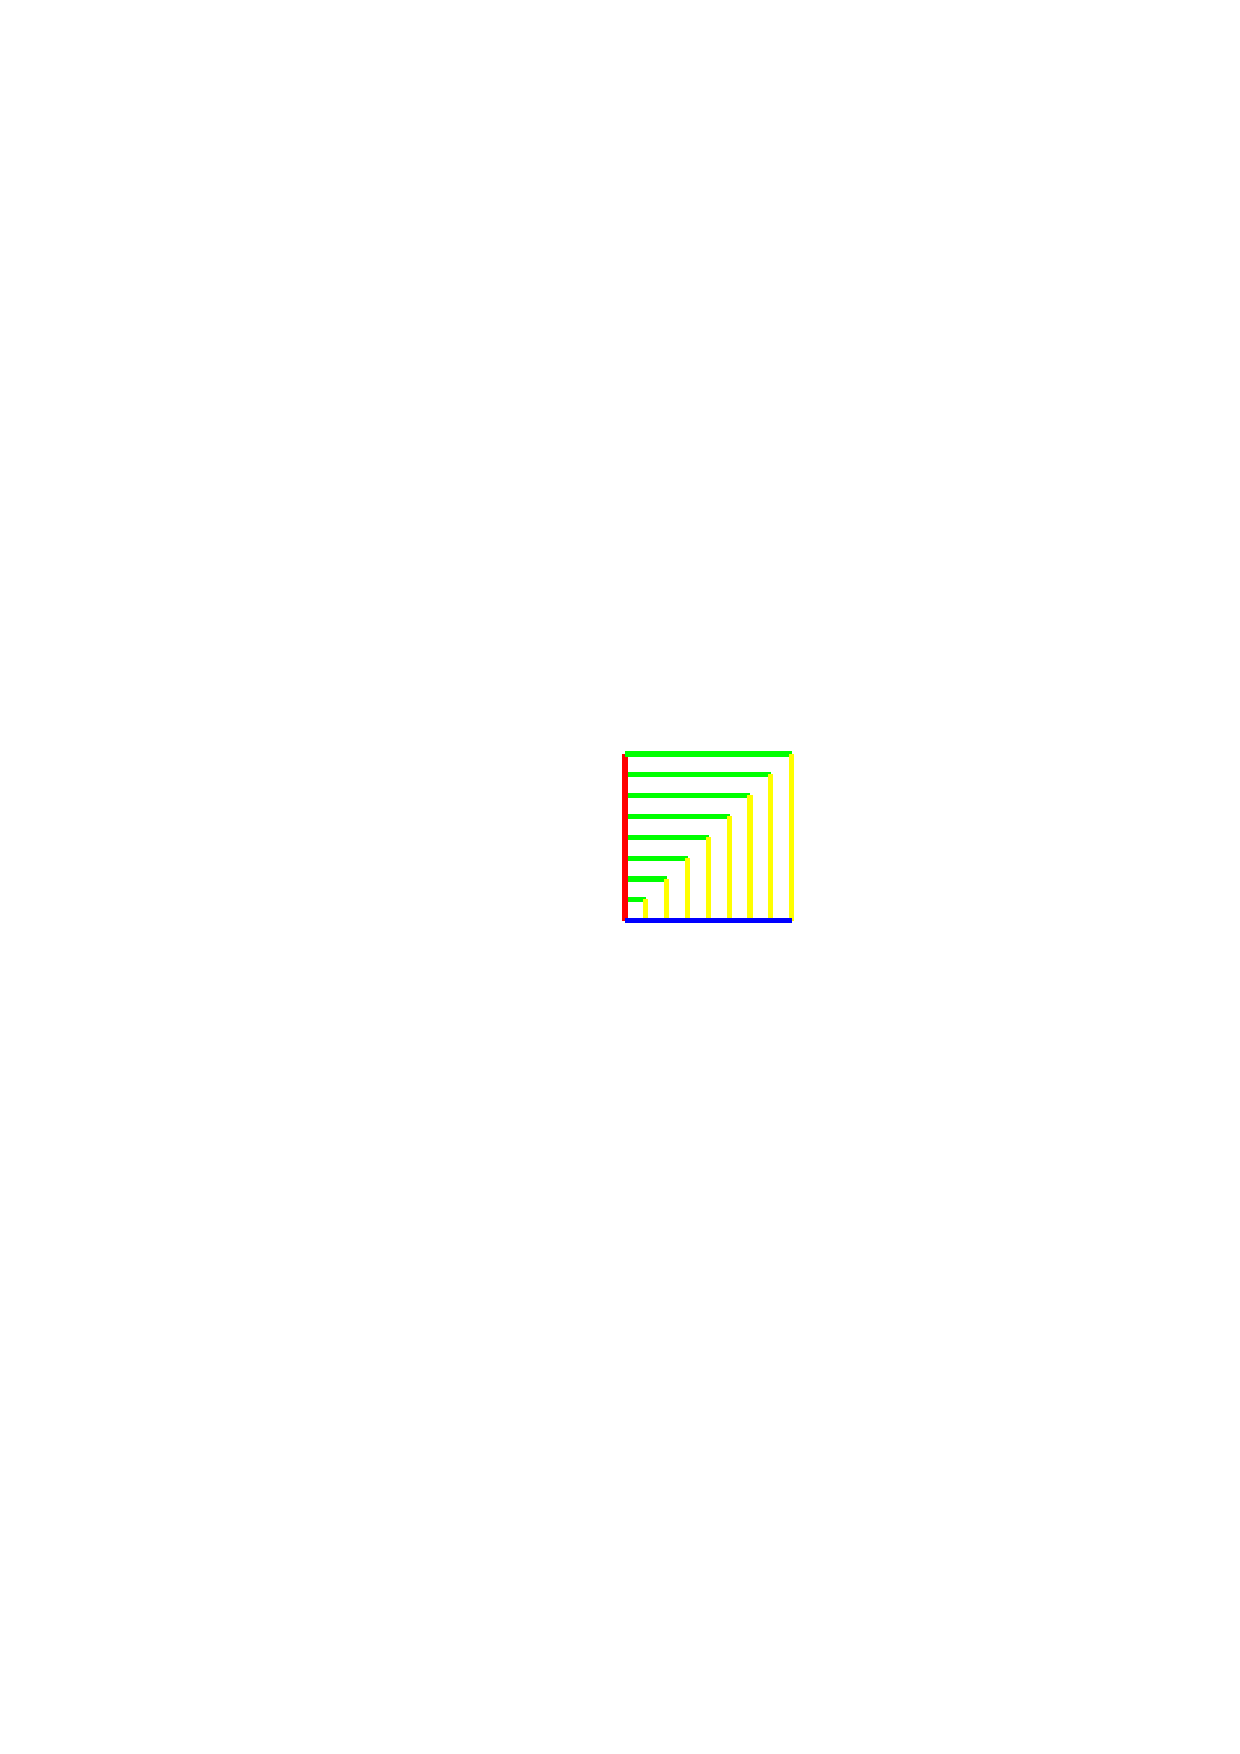
\includegraphics[clip,trim=10cm 11cm 6cm 11cm,scale=1.25]{../Pictures/out_tunnel.pdf}
\end{center}

\noindent Variables can be set using a postfix notation, e.g.~:
\begin{codesnippet}
START
   SET A ( 0 )
   SET B ( $A 1 + )
   SET C ( $B 2 * )
END
\end{codesnippet}

\subsection*{The Formal Grammar}
{\samepage
\begin{verbatim}
<PROG>   ::= "START" <INSLST>

<INSLST> ::= "END" | <INS> <INSLST>
<INS>    ::= <FWD> | <RGT> | <COL> | <LOOP> | <SET>

<FWD>    ::= "FORWARD" <VARNUM>
<RGT>    ::= "RIGHT" <VARNUM>
<COL>    ::= "COLOUR" <VAR> | "COLOUR" <WORD>
<LOOP>   ::= "LOOP" <LTR> "OVER" <LST> <INSLST>
<SET>    ::= "SET" <LTR> "(" <PFIX>

<VARNUM> ::= <VAR> | <NUM>
% Variables e.g. $A, $B, $Z etc.
<VAR>    ::= $<LTR>
% One Uppercase letter
<LTR>    ::= A, B ... Z
% Any valid double (as defined by scanf("%lf"...)
<NUM>    ::= 10 or -17.99 etc.

% A single word (as defined by scanf("%s"...) with double-quotes around it
% Valid colours include "BLACK", "RED", "GREEN", "BLUE",
% "YELLOW", "CYAN", "MAGENTA", "WHITE"
<WORD>   ::=  "RED", "BLUE", "HELLO!" or  "178"

<LST>    ::= "{" <ITEMS>
<ITEMS>  ::= "}" | <ITEM> <ITEMS>
<ITEM>   ::= <VARNUM> | <WORD>

<PFIX>   ::= ")" | <OP> <PFIX> | <VARNUM> <PFIX>
% A single mathematical operation character
<OP>     ::= + - / *
\end{verbatim}
}

\begin{exercise}

\strut\\[1em]
\vspace*{1ex}
\noindent{\bf\large Parser (35\%)}

\noindent Implement a recursive descent parser - this will report
whether or not a given turtle program follows the formal grammar or not.
The input file is specified via \verb^argv[1]^ - there is {\bf no}
output if the input file is {\bf valid}. Elsewise, a graceful non-zero
\verb^exit^ is made.  You should use the techniques described in the
lecture for this - writing code that carefully follows the grammar. For
instance, it won't use a tokenzier.

\noindent All source code will be in the \verb^Parse/^ sub-directory.

\vspace*{1em}
\noindent {\bf\large Interpreter (25\%)}

\noindent Extend the parser, so it becomes an interpreter. The
instructions are now `executed'. Do not begin a new program for this,
simply copy and then extend your existing parser. Output is to a text
file if the users specifies an \verb^argv[2]^, in the form of a 2D array
of characters where colours are represented by blac(K), (R)ed, (G)reen,
(Y)ellow, (B)lue, (M)agenta, (C)yan and (W)hite, via a $51$ wide $\times$
$33$ height array of characters e.g.:

\begin{verbatim}





                         GGGGGY
                         R    Y
                         R    Y
                         R    Y
                         R    Y
                      WWWWWWWWWWWW
                       W        W
                       W        W
                        W      W
                        W      W
                         W    W
                         W   W
                          W  W
                          W W
                           WW
                           W





\end{verbatim}

\noindent If no \verb^argv[2]^ is specified, then output is to the
screen using ANSI colour characters in same style as that used in
Section~\ref{sec:ansi}, with a $1$ second pause after each \verb^FORWARD^
instruction. 

\noindent Note that some files that successfully parse will not
successfully interpret (and vice versa) - there are example \verb^.ttl^
files provided to demonstrate this.

\noindent All interpreter source code will be in the \verb^Interp/^ sub-directory.

\vspace*{1em}
\noindent {\bf\large Postscript (5\%)}

\noindent Extend the output functionality of the
interpreter such that if \verb^argv[2]^ has a \verb^.ps^
extension, then the correct postscript instructions are written to that file.
\wwwurl{https://paulbourke.net/dataformats/postscript} Since PDFs are a
more common file format, then at the end, your program should also convert the \verb^.ps^
file to a \verb^.pdf^ file using a \verb^system()^ call in your C code
to \verb^ps2pdf^ which is installed on the lab machines. 
My implementation uses the postscript commands \verb^showpage^,
\verb^newpath^, \verb^moveto^, \verb^lineto^, \verb^setrgbcolour^, \verb^scale^
and \verb^stroke^.

If you get this to work, add it to the interpreter above - it will be tested
using both \verb^.txt^ and \verb^.ps^ output modes.

\vspace*{1ex}
\noindent {\bf\large Extension (15\%)}

\noindent Extend the project in a direction of
your choice. It should demonstrate your {\bf understanding} of some aspect
of programming or S/W engineering. If you extend the formal grammar
make sure that you give us the new, full grammar, along with the code in
the \verb^Extension/^ sub-directory named \verb^grammar.txt^, in addition to
a $300$ word (max) description of what you've achieve in \verb^extension.txt^.
Please do not submit ideas for future work, only functionality you've got working.

\vspace*{1ex}
\noindent {\bf\large Testing (20\%)}

\noindent Show the testing strategy on your code -
you should give details of any
unit testing or white/black-box testing done on your code. Describe any
test-harnesses used. Convince us that every line of your C code has
been tested, explaining the process, lessons learned and bugs found.
Submit a file \verb^testing.txt^ in the sub-directory \verb^Testing/^.

\subsection*{Hints}
\begin{itemize}

\item Understand the noughts and ones example given in the notes.

\item Don't try to write the entire program in one go. Try a cut
down version of the grammar first, e.g.:
{\small
\begin{verbatim}
<PROG>   ::= "START" <INSLST>

<INSLST> ::= "END" | <INS> <INSLST>
<INS>    ::= <FWD> | <RGT>

<FWD>    ::= "FORWARD" <NUM>
<RGT>    ::= "RIGHT" <NUM>

<NUM>    ::= 10 or -17.99 etc.
\end{verbatim}
}

\item The language is simply a sequence of words (even the braces),
so use \verb^fscanf()^.

\item Some issues, (e.g. drawing out-of-bounds), incorrect postfix
expressions cannot explained by the formal grammar. Use your own
common-sense to decide how to reconcile these, and explain what you
have done.

\item Once your parser works, extend it to become an interpreter. DO
NOT aim to parse the program first and then interpret it
separately. Interpreting and parsing are inseparably bound together. Use
our lectures notes for this and not those from other units such as
Architecture which take a very slightly different approach.

\item For the simple trigonometry required to compute the turtles
destination, bear in mind that the \verb^cos()^ and \verb^sin()^ functions
in C require parameters in radians and not degrees.

\item The turtle always begins in the centre of the screen facing due
north (upwards) and having a default white colour.  For the postscript/PDF
part, since white ink is hard to see on white paper, I've redefined
white ink to be slightly grey.

\item Start testing very early - this is a complex program to test and
trying to do it (or explain it) near the end won't work.

\end{itemize}

\subsection*{Submission}
Adapt the given Makefile if necessary to allow the parser, interpreter and extension to 
be built.
Submit your extension via text files \verb^extension.txt^ in \verb^Extension/^ along with  \verb^grammar.txt^ and your source code.

Your testing strategy will be explained in \verb^testing.txt^ along with any other files you'd like to bring our attention to in \verb^Testing/^.

Bundle this all up into a single \verb^turtle.zip file^ that contains {\bf everything} required
for us to compile and understand your code.

\end{exercise}
